\documentclass[a4j,12pt]{jarticle}
\usepackage[dvipdfmx]{graphicx}
\usepackage{amssymb}
\usepackage{amsmath}
\usepackage{float}
\usepackage{url}
\begin{document}
\begin{center}
\thispagestyle{empty}
\vspace*{5zh}
\huge
令和2年度 卒業論文\\[50pt]
{\Huge 論理的文章のアウトラインの作成を

支援するツールの開発}\\
[80pt]
\huge
指導教員 須田 宇宙 准教授\\[30pt]
千葉工業大学 情報ネットワーク学科\\[10pt]
須田研究室\\[60pt]
1632144 \hspace{70pt} 三浦 恋\\[75pt]
\end{center}
\vspace*{-2cm}
\begin{flushright} 
\huge
提出日 2020年1月--日
\end{flushright}

\newpage
\pagenumbering{roman}
\tableofcontents%目次
\newpage
\pagenumbering{arabic}
\section{緒言}
%目次を作る際は\verb+\tableofcontents+ と打ちます。\\
%新しいページに区切るときは\verb+\newpage+ と打ちます

%背景
大学生に対して,論理的な思考力や論理的文章作成能力の要求が高まっている.
しかし,論文やレポートを書く際にアウトラインなどの事前準備をせずに文章の作成を行ってしまう学生が多く,論理的な文章にならないことが問題点として挙げられる.
そのため,レポートの書き方の指導や修正を行うライティングセンターの設置などが進められているが
自発的に利用しなければ文章作成力は向上しない.

%問題点
一般に論文や小説などの長文を作成するためのツールとして,アウトラインプロセッサが使用されることが多い.
これは,文章を階層的に管理することに主眼が置かれており,学生にとって主張や根拠などが明確な一貫した文章を書く力を養うためのツールではないことが問題点となっている.

%目的
そこで本研究では,主張や根拠などが明確な一貫した文章を書く力を身に付け,論文やレポートの作成を支援するアカデミックアウトラインツールを開発することを目的としている.
\newpage
\section{アカデミックライティングについて}
\subsection{論文とは}
論文とはエッセイや小説のように自由な文章表現ではなく,一定の形式に備えた文章表現である.またテーマをもとに問題をたて,問題に対し様々な手法で,分析,考察し問題解決につながる新たな知見や検証を行い,その結果を報告するものが論文である\cite{ren1}.

\subsection{論文の書き方}
論文を書く流れとして主に4つ作業工程を繰り返し行うことで,より良い論文を書くことができる.また,4つの工程を以下に示す.
\begin{itemize}
  \item テーマを決める
  \item 下調べを行う
  \item アウトラインの作成する
  \item 執筆する
\end{itemize}
\subsubsection{テーマを決める}
論文のテーマを決める.素朴な疑問や資料を読んだ際の疑問を大切にし,どのような論文のテーマで書くのかを決める.またテーマが既に決まっている場合はキーワードをもとに,マップや表などを使って思考を整理し,論点を見出し下調べに入る.

\subsubsection{下調べを行う}
テーマに関しての知識を得ることを目的とし,検索エンジンや時点などで下調べを行う.文献等を調べる際は図書館での検索やデータベースによる検索をし,資料を収集する.また収集した資料を読み込み,疑問点などが出てきた際には2.2.1に戻りテーマや思考の整理を行う.論点が定まり,十分な情報が集まるまでテーマ決めと下調べを繰り返し行う.

\subsubsection{アウトラインの作成する}
論点をさだめ,文章の構造を組み立てるため,基本的な文章構成でもある序論,本論,結論,や章,節で書く内容や構成を組み立てる.そこでアウトラインを作成する際に紙に書き出すことやPCのメモ帳やアウトラインプロセッサなどのソフトウェアを使用したアウトラインの作成方法がある.アウトラインの作成例を図\ref{fig:a}に示す.

\subsubsection{執筆する}
定型的なフォーマットやアウトラインをもとに,執筆をする.アウトラインや整理した資料,行った実験や検証の結果をもとにアウトラインを更に細かく作成していく.そこで必要な情報があった際には調べ,アウトラインを修正し,執筆を行う.
また,文章の書き出しから完成まで,途中何度も書いた文章を添削,修正を行う必要がある.

\begin{figure}[h]
\begin{center}
 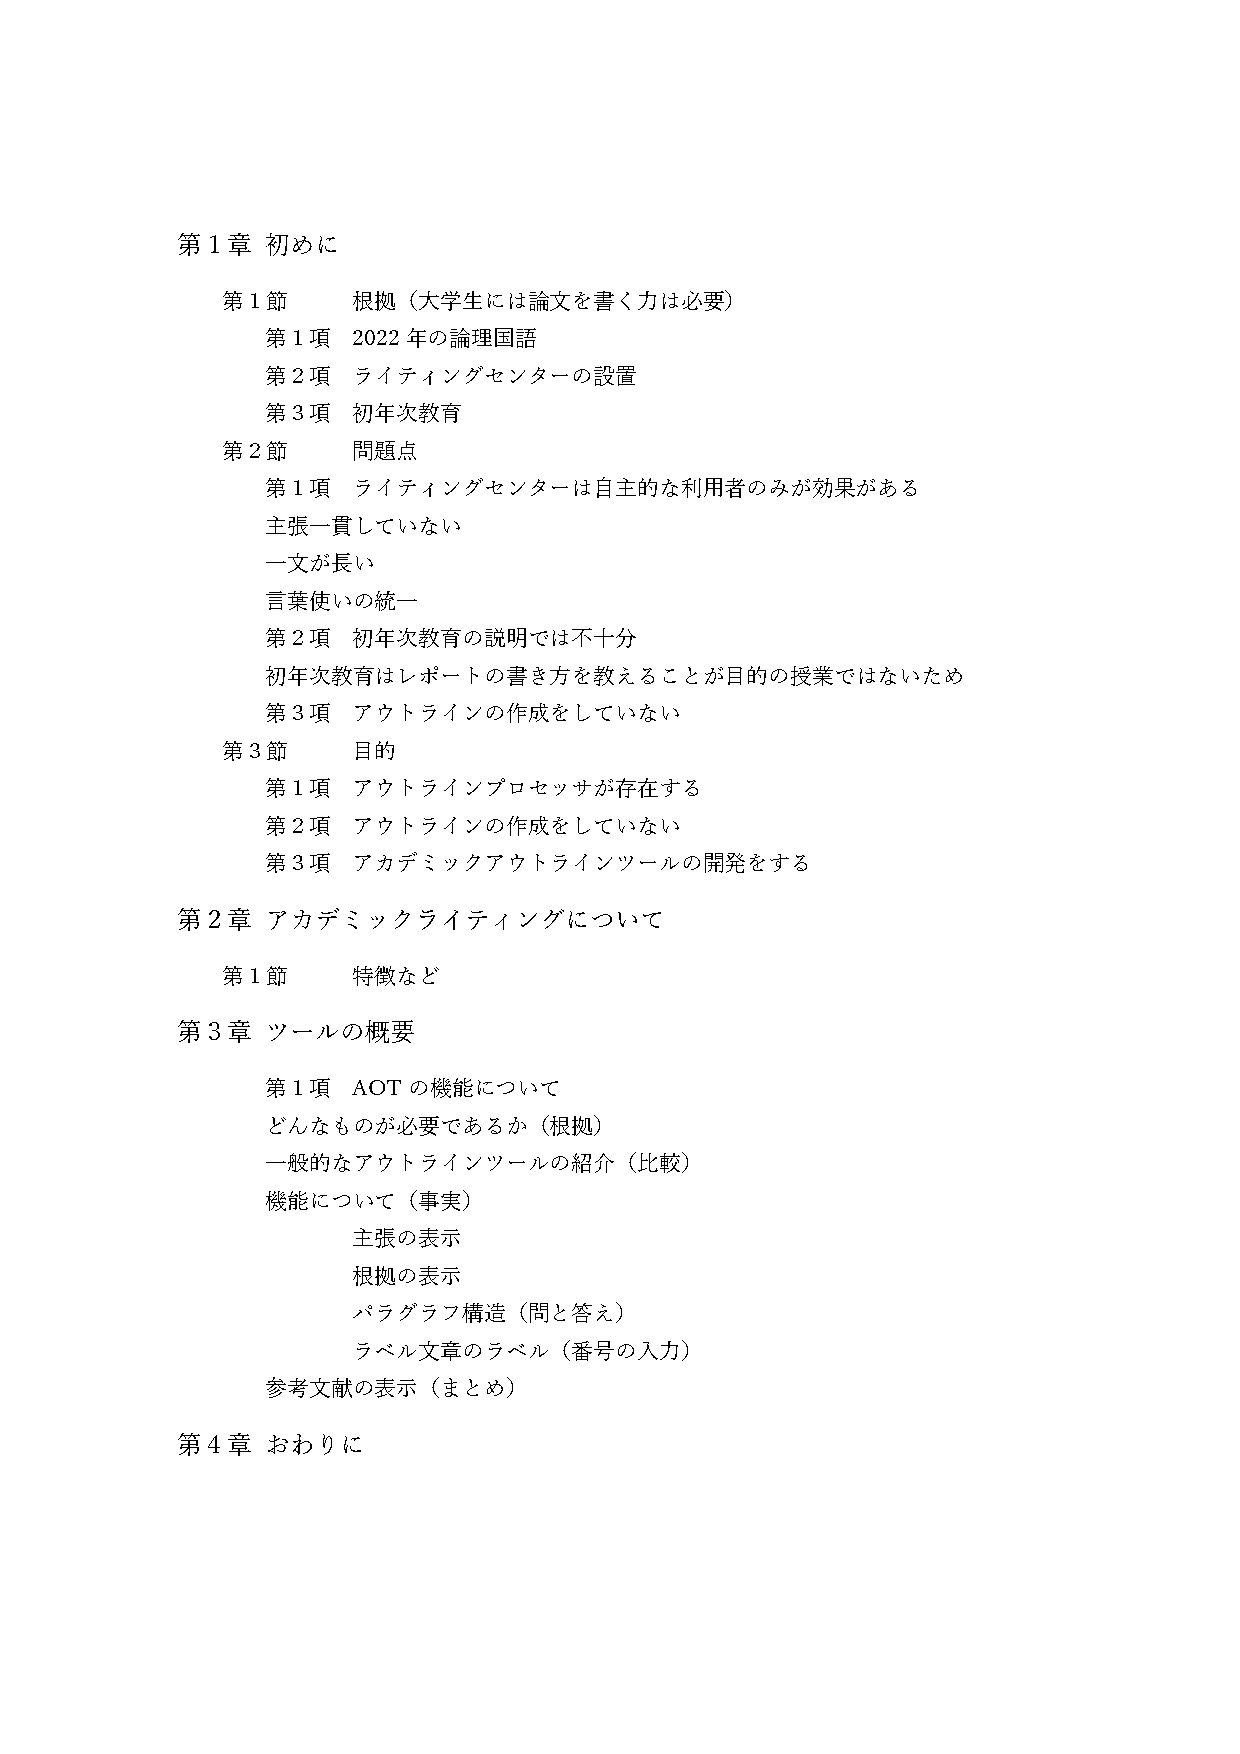
\includegraphics[scale=0.3]{outline.pdf}
\end{center}
 \caption{アウトラインの作成例}
 \label{fig:a}
\end{figure}
\newpage

\subsection{アカデミックライティングとは}
アカデミックライティングとは大学で作成が求められる,レポートや卒業論文や研究学術論文などの学術的な文章を書く技術または行為のことを指す\cite{ren2}.
\subsection{特徴}
アカデミックライティングには重要な特徴として,以下の(1)〜(5)が挙げられる.
\begin{description}
  \item[(1)] 主張と根拠が明示されている
  \item[(2)] 問いと答えの構造と論理的な説明での構成されている
  \item[(3)] 引用の倫理のルールに従っている
  \item[(4)] パラグラフ構造になっている
  \item[(5)] 学術的文章に特有の一定の形式に従ってる
 \end{description}

\newpage
\section{論文などの作成を支援するソフトウェアや手法の紹介}
\subsection{アウトラインプロセッサ}
アウトラインプロセッサとは,一般的には小説などの長文を書く際に利用されている.
特徴として,見出しをつけ階層的に管理や位置の入れ替えなど行い,全体の構成を確認しながら文章の作成を支援するソフトウェアである.
%図の挿入をする予定
\subsection{TEX}
TeXとは,アメリカの著名な数学者にして計算機科学者であるDonald E. Knuthが作成した組版フリーソフトウェアである.TeX本体は,文字を配置する,基本的な組版作業に対応する命令を処理するものであり,命令だけを用いて文書を作成するのは効率的ではない.そこで多くの場合マクロセットと呼ばれる命令セットを用いて文書を作成している.

マクロとは,組版された文書の作成を容易にするために,複数の基本的な命令を組み合わせて作成された新たな命令である.
マクロセットにはさまざまなものがあるが,もっとも有名でよく用いられているものが,アメリカの計算機科学者であるLeslieLamportが作成したLaTeXである.TeXで文書を作成するという場合,実際はこのLaTeXの命令を用いて作成することがほとんどである.

また,日本語で書かれた文章をTeXで組版するため,(株)アスキーにおいてASCII日本語TeXが,日本電信電話公社においてNTT JTeXがそれぞれ開発されたことにより,日本においてもTeXが普及し現在に至っている\cite{ren3}.
%図の挿入をする予定

\subsection{Microsoft Word}
WordとはMicrosoft社が提供する文章作成ソフトウェアである.Micosoft社がが販売するワープロソフトのことであり,ソフトウェアのパッケージ製品であるMicrosoft Officeの中でも,主要なソフトウェアの1つに挙げられる.また,文章作成だけでなく,図形描画やグラフ,アウトラインの作成など,豊富で様々な機能のを持つ.
%図の挿入をする予定?いる?
\newpage
\subsection{マインドマップ}
マインドマップとは,頭の中で自然に行っている思考のプロセスを反映したノート法である.イギリス人教育者であるトニー・ブザン (Tony Buzan)が1970年代に出演していたTV番組を始めとして様々な著作で「マインドマップ」という言葉が広め始めた\cite{ren4}.また,自由な思考,アイデアや情報の流れを中心となる概念から分岐させる形で描画した図である.描画することで,アイデアの整理,効果的なメモの作成,記憶の定着強化などを実現することが可能になる.書き方として以下の6つの法則がある\cite{ren5}.
\subsubsection{無地の用紙}
  マインドマップを書く際には無地の用紙を用いる.罫線がある場合,無意識に罫線に影響を受け,思考の自由度がなくなってしまうため無地の用紙を利用をする.
\subsubsection{線}
 中央のイメージから放射状に多くの線を伸ばしていき,その線を「ブランチ (枝)」と呼ぶ.木の枝のように,枝同士がつながり,外側に向かって分岐していく事により自由な連想によりアイデアを出すことができる.また基本的にはマインドマップ内での枝は「曲線」で描く.
\subsubsection{言葉}
連想する際に,枝の上側に言葉またはイメージを載せていく.短い文章で書くことにより,枝と枝の関連性を把握することができる.また短い文章に分割して書くことで,思い出しやすい.
\subsubsection{イメージ}
脳は言葉よりもイメージに素早く反応することや1つのイメージは,10個の言葉以上の情報を持っており,記憶にも残りやすいため,全体にイメージを入れるようにする.そのため視覚的な表現力を磨き,マインドマップの各所にイメージを入れるようにする.
\subsubsection{カラー}
 分類や重要な部分を目立たせることができるため複数の色を使い分けることが必要とされている.
 色分けをすることで,同じ塊を一目で認識できることや.違う色は異なる内容で有ることを直感的に把握することができるため色を使い分ける.
\subsubsection{構造}
脳が自然に行っている連想をそのまま表現するノート法であるが,論理性や構造を排除しているものでなく,思考を構造的にまとめていくことも必要である.しかし構造にこだわり過ぎてしまうと自然な連想が止る場合もあるため,構造化だけに捉われないように作成をする.
%mainndomap zu 



\newpage
\section{実装技術}
\subsection{PWAとは}
PWA(Progressive Web Apps)とはモバイルサイト上でネイティブアプリのようなユーザー体験を提供する技術であり,ウェブとアプリの両方の良さを兼ね備えている.具体的にはインストールが必要なく,ホーム画面へのアイコン追加やプッシュ通知の可能であり,ユーザーとの接触機会を増やすことができる.また読み込み速度や表示の高速化,オフラインでの閲覧も可能であるなど様々なメリットが得られる.またアプリとの違いとして,アプリストアを経由してダウンロードやインストールする手間がなく,アプリの導入までの手順を短縮ができる.またプラットフォームごとに開発する必要も
なく1つのPWAを構築するだけで,デバイスを問わずに一貫した内容を表示できるなど開発の自由度が高い\cite{ren6}.
\newpage
\section{本研究で開発したツールの概要}
\subsection{実装理由}
%実装した機能がなぜひつようであるのか?コンセプトを書く
本制作では論理的文章を書く際に準備段階であるアウトラインの作成において,主張と根拠の確認や参考文献の管理を行うことでアウトラインの作成や主張の一貫した文章の作成を支援することができるツールが必要であると考えた.また,通学時間などの隙間時間で意見や構成の整理を行うことでアウトラインの作成時間を短くし,論理的文章を書く時間の確保ができることを目指した.

\subsection{開発言語について}
開発言語として,自宅や学校のみならず隙間時間に利用することを視野に入れ,PC とスマートフォンの両
方からのアクセスによる利用を考えた.そこで Web 上で動作するツールが望ましいと考え,HTML5,CSS3, JavaScript を使用し開発を行った.
\subsection{実装した機能について}
本ツールで開発した機能は以下の4つの機能の開発を行った.
\begin{description}
  \item[(1)] 主張と根拠の明確化
  \item[(2)] 課題に対する疑問とその答えの記入
  \item[(3)] 論理的な構成の整理
  \item[(4)] 参考文献の管理
 \end{description}
%実際の画面を画像としてはる
\subsubsection{主張と根拠の明確化}
主張と根拠を明確にする機能は,文章作成時や添削等を行う際に主張や根拠の確認を行うことで,主張からずれた意見が出ることを防ぐことや添削の際にずれた意見を見つけやすくする機能にした. 
\subsubsection{課題に対する疑問とその答えの記入}
この機能では文章の内容をアカデミックライティングの特徴である「問いと答え」の形式に従って記述を行うことで,文章に必要な情報などを明確化していくことができると考えこのような機能にした.
\subsubsection{論理的な構成の整理}
この機能では,一般的なアウトラインプロセッサと同様に論理的な文章を書く上で各内容の順番や情報を整理するため順番を入れ替える機能,章や段落の情報を表示する機能
\subsubsection{参考文献の管理}
文章を作成する際に引用した文献を確認, 整理する機能
\subsection{利用方法}
%図を使っての利用方法の説明を行う.

\newpage

\section*{謝辞}

\addcontentsline{toc}{section}{謝辞}
ここに研究の謝辞.主にご協力いただいた方など.
\bibliographystyle{jplain}
\newpage
\addcontentsline{toc}{section}{参考文献}
 \begin{thebibliography}{99}
\bibitem{ren1}山崎 憲一,萬代 雅希"論文とは",電子情報通信学会 通信ソサイエティマガジン,2016年9巻4号216-221.
\url{https://www.jstage.jst.go.jp/article/bplus/9/4/9_216/_pdf}

\bibitem{ren2} 堀 一成,坂尻 彰宏:"阪大生のためのアカデミックライティング",
\url{https://ir.library.osaka-u.ac.jp/repo/ouka/all/27153/Academic%20Writing%20Introduction.pdf}, 2019/8/23参照
\bibitem{ren3} 山本 浩: "TeXを使った論文作成方法",2000年103巻984号770-773.
\url{https://www.jstage.jst.go.jp/article/jsmemag/103/984/103_KJ00001459868/_article/-char/ja/}
\bibitem{ren4} "Lucidchart,5分でわかる、マインドマップの書き方と意味"
\url{https://www.lucidchart.com/pages/ja/mind-map#section_0}
\bibitem{ren5} "マインドマップの学校"
\url{https://www.mindmap-school.jp/mindmap/mindmap-law/}
\bibitem{ren6} "ディーエムソリューションズ株式会社"
\url{https://digital-marketing.jp/seo/what-is-progressive-web-apps/#i-6}

\end{thebibliography}
\section*{付録}

\addcontentsline{toc}{section}{付録}

\end{document}
